% !TeX spellcheck = de_DE
\section{Optimierungsprobleme}
\label{sec:analysis_optimzation_problems}
Nach erfolgreicher Verifizierung der Funktionalität wird in diesem Kapitel auf verschiedene andere Optimierungsprobleme eingegangen, anhand derer die Analyse durchgeführt werden soll. Grundsätzlich ist bei der Implementierung zu beachten, dass keine zu aufwendigen Optimierungsprobleme verwendet werden, da der Raspberry Pi 4 nicht so leistungsfähig ist und die benötigte Optimierungszeit sehr hoch sein kann. Daher werden im Folgenden hauptsächlich klassische Probleme des bestärkenden Lernens aus dem OpenAI Gym verwendet. Die ausgewählten Umgebungen sind das \emph{Cartpole}, \emph{MountainCar} und das \emph{Pendulum} Problem. Im Folgenden wird auf die entsprechenden Optimierungsprobleme genauer eingegangen und die Implementierung der Fitnessfunktion und Abbruchbedingung vorgestellt. 

\subsection{Cartpole}
Die \emph{Cartpole} Umgebung, auch als \emph{Pole Balancing} bezeichnet, wurde bereits 1983 das erste mal in Quelle \cite{barto1983neuronlike} vorgestellt und ist auch heute noch ein bekanntes Optimierungsproblem, welches in vielen Publikationen verwendet wird. Auch im OpenAI Gym ist dieses Problem entsprechend der Beschreibung aus Quelle \cite{barto1983neuronlike} enthalten und in Abbildung \ref{fig:cartpole_environment} dargestellt. In der Umgebung befinden sich zwei Gegenstände. Das erste ist ein Wagen, welcher vom Agenten nach links und rechts bewegt werden kann. Hierauf befindet sich ein Balken, der am unteren Ende mit dem Wagen verbunden ist. Entsprechend seiner Position kann dieser nach links oder rechts kippen. Ziel des Agenten ist, durch Steuerung des Wagens den Balken so lange wie möglich senkrecht zu balancieren. Bezüglich der Abbruchbedingung gilt, dass der Agent scheitert, wenn  sich der Balken um mehr als 15 Grad zur Seite neigt oder der Wagen zu weit vom Zentrum entfernt ist. Als Eingabewerte für das \ac{KNN} werden von der Umgebung vier Werte zur Verfügung gestellt, für welche je ein Eingabeneuron erstellt wird. Dies ist unter anderem die Position und Geschwindigkeit des Wagens, der aktuelle Winkel des Balkens und dessen Änderungsrate. Zusätzlich besitzt das erstellte \ac{KNN} zwei Ausgabeneuronen, welche die jeweilige Richtung repräsentieren. Ist der Aktivierungsgrad des erstens \emph{Output}-Neurons höher als der des zweiten, wird der Wagen nach links bewegt und andernfalls nach rechts.
\begin{figure}[!h]
	\centering
	
\includegraphics[width=0.5\textwidth]{./img/cartpole_env.JPG} 
	\caption{Darstellung der \emph{Cartpole} Umgebung aus dem OpenAI Gym}
	\label{fig:cartpole_environment}
\end{figure} 
Bevor die Evaluation mit dieser Umgebung durchgeführt wird, müssen die Fitnessfunktion, Lösungsbedingung und Konfiguration festgelegt werden. Beim klassischen bestärkenden Lernen, wie in Kapitel \ref{subsubsec:reinforcment_learning} beschrieben, erhält der Agent nach jedem Zeitschritt einen \emph{reward}. Da das OpenAI Gym primär für diese Art des Lernens konzipiert ist, wird auch hier nach jeder Aktion in der Umgebung ein \emph{reward} zurückgegeben. In diesem Fall erhält ein Agent bis zum Scheitern für jeden Zeitschritt einen \emph{reward} mit der Wertigkeit $1$. Mit diesen muss für neuroevolutionäre Algorithmen eine Fitnessfunktion definiert werden. Bei diesem Beispiel ist das Vorgehen einfach. Der Fitnesswert wird berechnet, indem die erhaltenen \emph{rewards} aggregiert und der resultierende Wert am Ende der Evaluation quadriert wird. Somit soll wie zuvor beim XOR-Problem besseren Agenten ein proportional höherer Fitnesswert zugewiesen werden. Das Optimierungsverfahren wird beendet, wenn ein Agent den Balken 500 Zeitschritte balancieren kann. Die restlichen Parameter wurden aus dem vorherigen Beispiel übernommen und nicht geändert.
\begin{figure}[!h]
	\centering
	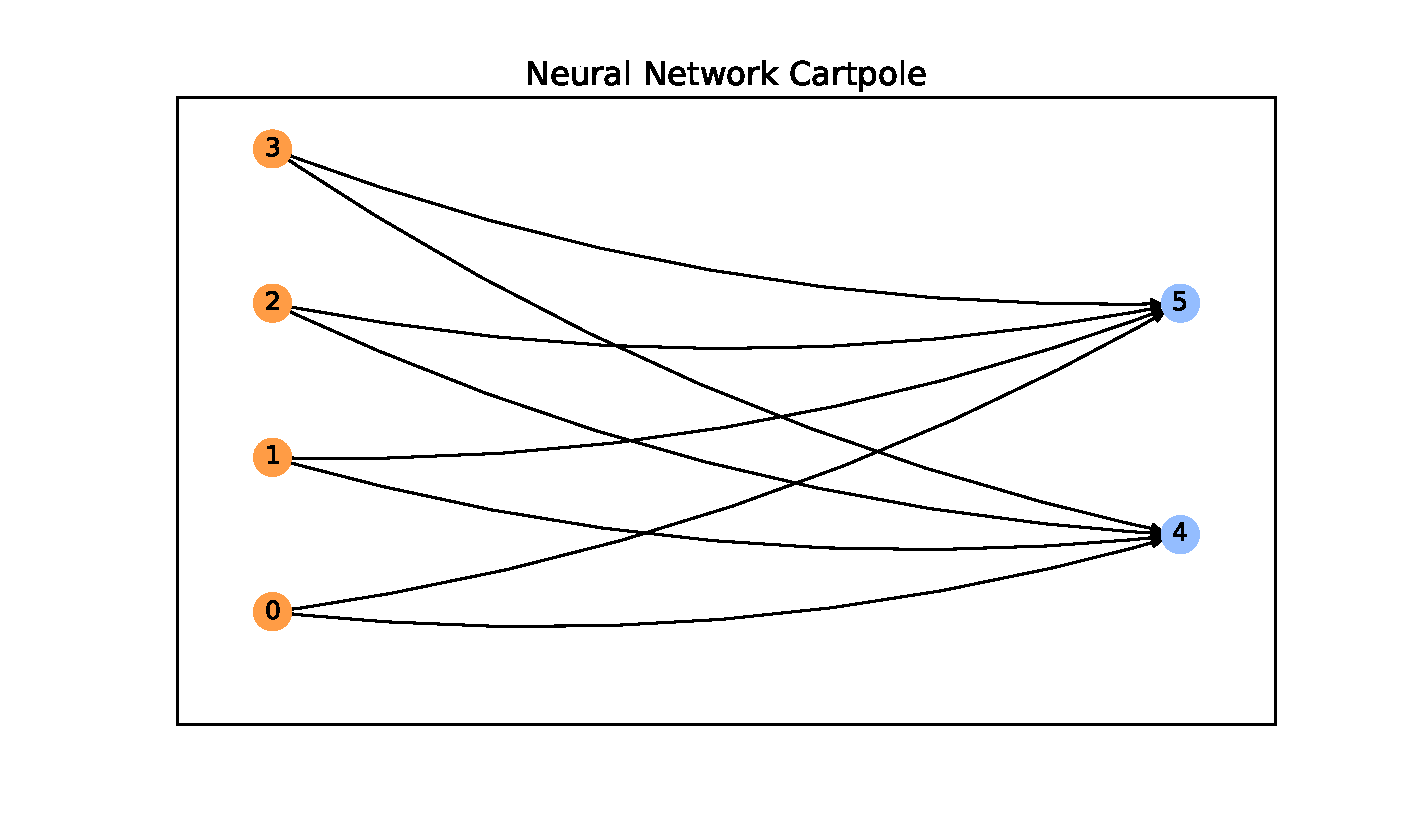
\includegraphics[width=0.7\textwidth]{./img/pole_balancing_single_core/cartpole_neuroal_network.pdf} 
	\caption{Struktur des finalen KNN im \emph{Cartpole} Optimierungsproblem}
	\label{fig:cartpole_neural_network}
\end{figure}
\\\\
Allerdings stellt sich beim Ausführen dieses Optimierungsproblems heraus, dass es für die Analyse ungeeignet ist. Bereits bei den zufällig erstellten Agenten der initialen Population, sind \ac{KNN} vorhanden, welche die Abbruchbedingung erfüllen und das Optimierungsproblem lösen. Ein solches ist in Abbildung \ref{fig:cartpole_neural_network} dargestellt. Wie die anderen \ac{KNN} in der initialen Population besitzt auch dieses keine \emph{Hidden}-Neuronen und zeigt, dass für das Lösen dieses Optimierungsproblems keine komplexen Entscheidungen notwendig sind. Es ist beispielsweise möglich, mit dem Winkel des Balkens auf die auszuführende Aktion zu schließen. Neigt sich der Balken nach rechts, bewegt sich der Wagen in diese Richtung und umgekehrt. Dies ist einer der Gründe, warum dieses Optimierungsproblem im weiteren Verlauf der Arbeit nicht weiter verwendet wird. Ein weiterer Grund ist, dass aufgrund der fehlenden keine Ausführungszeiten über mehrere Generationen gemessen werden können, welche eine notwendige Grundlage für den späteren Vergleich sind.

\subsection{Mountain Car}
Die Umgebung \emph{Mountain Car} ist ein weiteres Optimierungsproblem, welches aus dem OpenAI Gym stammt und in Abbildung \ref{fig:mountain_car_env} dargestellt ist. Das Ziel für den Agenten ist, den Wagen auf den rechten Berg zu fahren, auf welchem sich die Fahne befindet. Hierfür stehen ihm Steuerungsoptionen für den Antrieb des Wagens zur Verfügung. Für jeden Zeitschritt kann der Agent entscheiden, ob er nach links, rechts oder gar nicht beschleunigen möchte. Die Schwierigkeit von dieser Umgebung ist, dass der Antrieb nicht ausreichen ist, um den Wagen zur rechten Bergspitze zu fahren. Das Ziel kann nur erreicht werden, wenn der Wagen zuerst ein Stück den linken Berg hochfährt. Ab einer gewissen Höhe kann in die andere Richtung beschleunigt werden und mit dem zusätzlichen Schwung kann der Wagen letztendlich die rechte Bergspitze erreichen. Für dieses Optimierungsproblem gibt es zwei Eingabewerte. Der erste ist die aktuelle Position des Wagens und die zweite seine Geschwindigkeit. Auf Basis von diesen muss der Agent seine Aktion wählen. Auch für diese Umgebung muss eine Abbruchbedingung und Fitnessfunktion festgelegt werden. Die Ausführung der Umgebung wird beendet, wenn der Agent entweder das Ziel auf der rechten Seite erreicht hat oder wenn $200$ Zeitschritte vergangen sind. Das erreichen der Fahne allein ist nicht ausreichend um das \emph{Mountain Car} Problem erfolgreich zu lösen. Laut der Dokumentation des OpenAI Gyms muss der Agent dies in $100$ aufeinander folgenden Evaluationen in durchschnittlich $110$ Zeitschritten oder weniger schaffen.
\begin{figure}[!h]
	\centering
	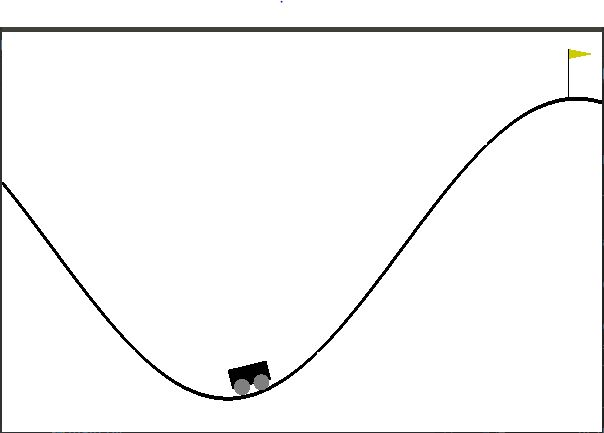
\includegraphics[width=0.5\textwidth]{./img/mountain_car_env.JPG} 
	\caption{Darstellung der \emph{Mountain Car} Umgebung aus dem OpenAI Gym}
	\label{fig:mountain_car_env}
\end{figure} 
\\\\
Grundsätzlich kann dies implementiert werden, indem beispielsweise nach jeder Generation der beste Agent $100$ mal in verschiedenen Umgebungen getestet wird. Aber da dies die Trainingszeit stark erhöhen würde, und die Laufzeit auf dem Raspberry Pi 4 vergleichsweise hoch ist, wird eine einfachere Bedingung gewählt. Das Trainingsverfahren wird beendet, wenn es einem Agenten einmalig gelingt, das \emph{Mountain Car} Problem in weniger als $110$ Zeitschritten erfolgreich zu beenden. Zuletzt muss die Fitnessfunktion implementiert werden. Die \emph{Mountain Car} Umgebung gibt für jeden Zeitschritt einen \emph{reward} von $-1$. Für eine bessere Übersichtlichkeit und um negative Fitnesswerte zu vermeiden, wird der Fitnesswert in dieser Umgebung auf den $200$ initialisiert. Für jeden verwendeten Zeitschritt wird ein Punkt abgezogen. Bessere Agenten, welche weniger Zeitschritte benötigten, haben so einen höheren Fitnesswert. Allerdings kann vorkommen, dass kein Agent in der initialen Population das Ziel auf der rechten Seite erreicht. In diesem Fall würde jeder Agent den Fitnesswert $0$ haben, wodurch keine Selektion möglich ist. Aus diesem Grund wird die maximal erreichte X-Koordinate ebenfalls in den Fitnesswert miteinbezogen. Sollte kein Agent das Ziel erreichen, haben die Agenten, welche diesem am nächsten waren einen Selektionsvorteil. Die restliche Konfiguration für diese Umgebung ist sehr ähnlich zu den vorherigen Beispielen. Einzig die Populationsgröße wird auf $300$ Agenten erhöht, da dieses Problem aufwändiger zu lösen ist als die vorherigen.
\\\\
Prinzipiell kann das Verfahren ab diesem Punkt evaluiert werden, allerdings werden die maximalen Fitnesswerte in vielen Fällen stark variieren. Der Grund hierfür ist eine verrauschte Fitnessfunktion, wie es in Kapitel \ref{subsec:comparision_neuroevoltion} erläutert ist. Die Startposition des Wagen ist zufällige durch die Umgebung gesetzt und kann einen großen Einfluss auf den Fitnesswert haben. So kann es vorkommen, dass ein Agent einen hohen Fitnesswert durch eine günstige Startposition erhält aber ansonsten schlechte Ergebnisse erzielen würde. Ein Ansatz um diesen Effekt zu minimieren ist, dass jeder Agent mehrfach die Evaluation durchführen muss und der mittlere Fitnesswert verwendet wird. Aber da dies die Trainingszeit weiter stark erhöhen würde und nicht für einen Vergleich zwischen der sequenziellen und parallelisierten Implementierung notwendig ist, wird hierauf verzichtet. Stattdessen wird die Umgebungen so konfiguriert, dass jeder Agent mit derselben Ausgangssituation beginnt. 
\begin{figure}[!h]
	\centering
	\begin{minipage}[]{0.49\textwidth}
		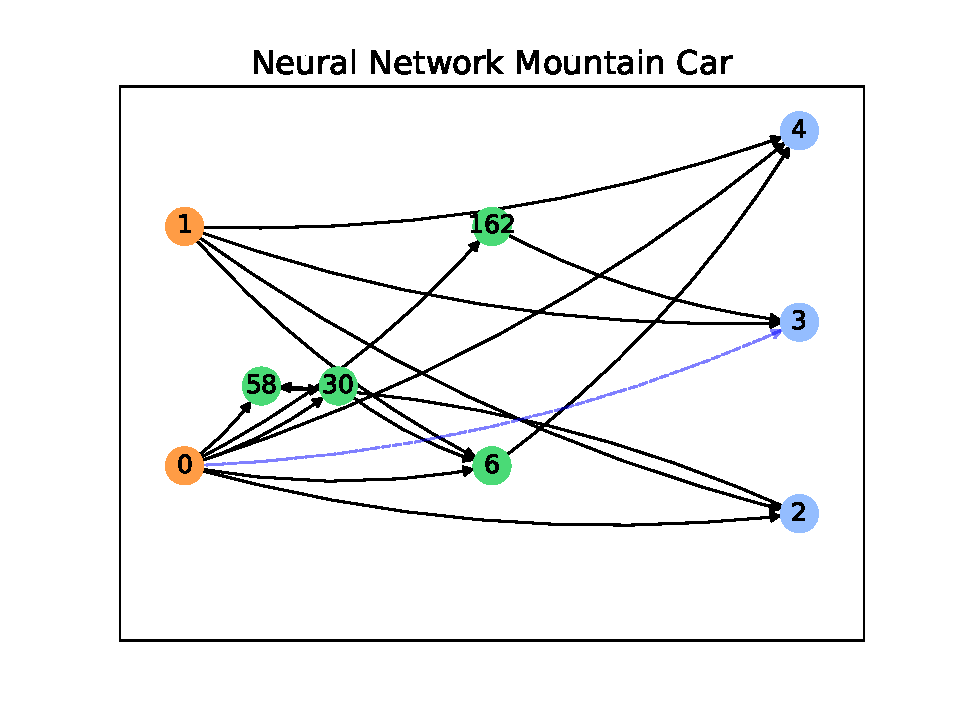
\includegraphics[width=1.0\textwidth]{./img/mountain_car_single/mountain_car_neural_network.pdf} 
		%\caption{Lösung für das XOR-Problem mit einem \emph{Hidden}-Neuron}
		%\label{fig:xor_solution_minimal}
	\end{minipage}
	\hfill
	\begin{minipage}[]{0.49\textwidth}
		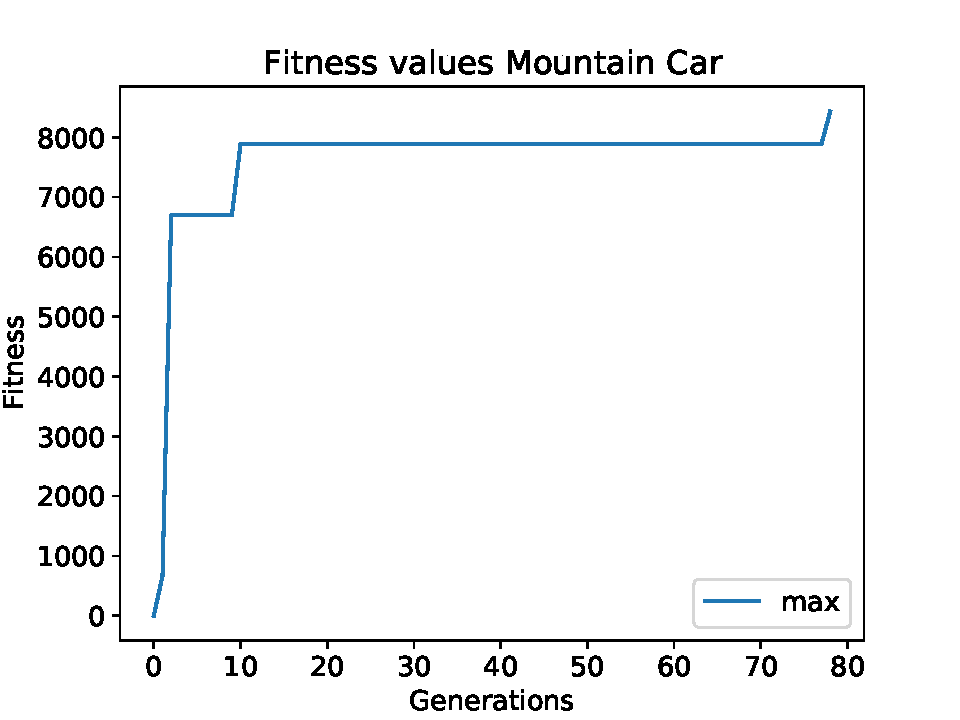
\includegraphics[width=1.0\textwidth]{./img/mountain_car_single/1413_fitness_1core_1pi.pdf} 
		%\caption{Lösung für das XOR-Problem mit einem \emph{Hidden}-Neuron}
	\end{minipage}
	\caption{Links die Lösung für das Mountain Car Problem, rechts die dazugehörigen Fitnesswerte pro Generation}
	\label{fig:mountain_car_1core_neural_network_and_fitness}
\end{figure}
\\\\
\begin{figure}[!h]
	\centering
	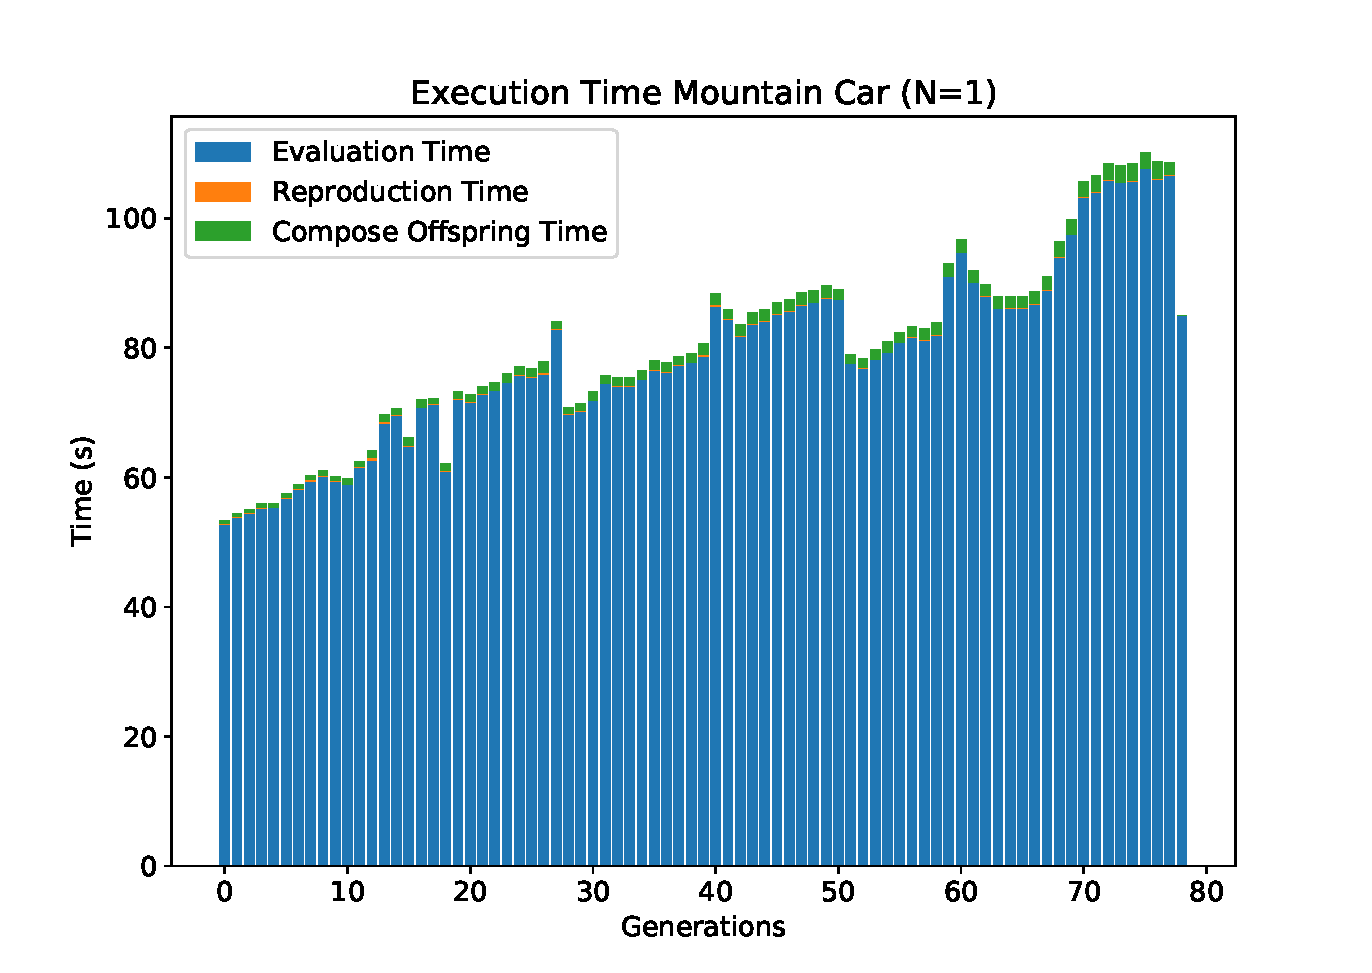
\includegraphics[width=0.7\textwidth]{./img/mountain_car_single/1413_time_1core_1pi.pdf} 
	\caption{Ausführungszeiten des Mountain Car Problems auf einem Raspberry Pi 4 mit einem Prozess}
	\label{fig:mountain_car_time_single_core}
\end{figure}

% Time ca: 105 Min

% Recurrent Verbindungen?
% Ergebnisse

\subsection{Pendulum}


